% generated by make_combined.py from stage6_remedies_audit_paper/stage6.tex; do not edit
\section{Stage 6 --- What to do instead of masking, and the state of the thesis}\label{sec:stage6}

\stagebox{\textbf{In one sentence.} What to use instead of masking depends on what carries the shortcut: an
annotation-free mask-then-erase method (U-MtE) repairs artifacts that carry the shortcut in their own pixels (calipers:
thyroid Trap~A \sSixRemThyroidmte{} versus ERM, masking \sSixRemThyroidmask), needs a disease-protection step when the
artifact resembles the pathology (capsule debris), and cannot help when the shortcut is carried by correlates of the
artifact (hair, chest drains), where only label-based reweighting works; with image-level artifact labels, U-MtE with
balancing or masking with DFR is the most robust choice; for fully fine-tuned networks erasure must happen during
training; and no remedy improves on masking uniformly on unaltered data. The thesis manuscript, its number audit, the
CLAIM checklist and a blinded clinician audit package are ready; the audit itself has not been performed.}
\subsection{Where this stage starts}
Stages~1--5 established that ROI masking removes an artifact outside the ROI and concentrates the model on one inside
it; that this is caused by location, not by which images carry the artifact; that it matters on unaltered data and at
clinical operating points; and that a two-parameter model explains it. They also showed three facts that shape any
remedy: label-based methods (balancing, DFR) fix both locations but need image-level artifact labels; removing the
artifact's pixels fails when the artifact resembles the disease (capsule debris); and some shortcuts are carried by
correlates of the artifact rather than its pixels (hair, drains). This stage asks what a practitioner should do instead
of masking, and reports the state of the thesis.

\subsection{Questions}
\begin{enumerate}[label=\textbf{Q6\alph*},leftmargin=*]\itemsep1pt
\item Can an in-ROI shortcut be removed from frozen foundation-model features \emph{without} any artifact annotation ---
no artifact example, mask or label, only the ROI mask that masking already uses?
\item When does such a remedy fail, and which alternative fits which regime?
\item Can the same be done for networks fine-tuned end to end?
\item Does any remedy transfer to unaltered test data?
\item How will the automatic artifact labels be validated by a clinician, and what remains before submission?
\end{enumerate}

\subsection{Method: from insert-then-erase to U-MtE}\label{s6:sec:method}
\paragraph{Idea} Masking leaves exactly one thing to remove: what lies inside the ROI and is not disease. If we knew
the directions in feature space along which an artifact moves an image, we could project them out. The method estimates
those directions by \emph{inserting} artifacts into images and measuring how the features change.
\paragraph{Evolution}
\begin{enumerate}[leftmargin=*]\itemsep1pt
\item \textbf{Insert-then-erase (I2E).} Paste artifact \emph{templates} (e.g.\ real hair strands cut from other images)
into training images, collect the paired feature differences (with minus without), take the subspace $U_k$ holding 90\%
of their held-out energy (cap 64 directions), and erase it: $x\mapsto x-U_kU_k^\top(x-\mu)$; a logistic head is trained on
the erased features. Works, but needs examples of the artifact.
\item \textbf{Mask-then-erase (MtE).} Estimate the subspace on \emph{masked} images (insert, then mask), so that erasure
targets exactly what masking leaves; the head is trained and tested on masked, erased features.
\item \textbf{U-MtE (universal).} Replace the templates by one \emph{generic} procedural overlay library --- thin strokes,
thick bands, solid and translucent patches, blobs, dashed lines, small glyphs; random colour (half grey), opacity,
width and position, half centred in the ROI (Figure~\ref{s6:fig:overlays}) --- used \emph{unchanged} for every artifact,
dataset and modality. It contains no ruler, no caliper and no hair. U-MtE needs no artifact example, mask or label; only
the ROI mask.
\item \textbf{Disease protection.} If the erased subspace overlaps the disease direction, erasure removes disease
evidence. Protection estimates label directions $W$ on the \emph{artifact-free} training images and erases
$\mathrm{orth}\big((I-WW^\top)U_k\big)$, which leaves every protected direction untouched ($w^\top P(x)=w^\top x$). It
needs diagnosis labels of artifact-free images (which any training set has) and no artifact label.
\item \textbf{U-MtE with balancing.} When image-level artifact labels exist, the head is group-balanced.
\end{enumerate}
\paragraph{Why it should work (theory of Stage~5)} Erasure sets the effective artifact signal $\tilde A$ to zero but scales
the disease signal by $1-\rho^2$, where $\rho$ is the overlap between the erased subspace and the disease direction. It
therefore beats in-ROI masking unless $\rho$ is large --- which is the case when the artifact resembles the disease, and
which protection forces to zero along the protected directions. Overlay \emph{augmentation} with the same overlays only
decorrelates the label from the generated overlays, not from the real artifact; erasure removes the whole subspace of
``foreign overlay'' changes, which contains the real artifact's direction when both move the representation in shared
ways. The theory therefore predicts erase $\gg$ augment for overlay-like artifacts.
\begin{figure}[H]\centering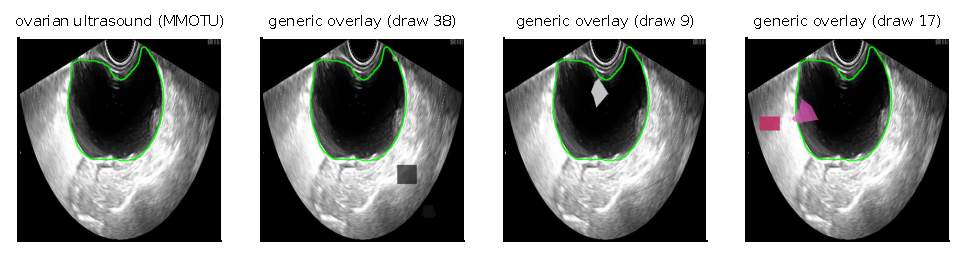
\includegraphics[width=0.9\linewidth]{../stage6_remedies_audit_paper/figures/overlays.pdf}
\caption{The generic overlay library (the same for every modality) drawn on an ovarian ultrasound image (MMOTU, CC BY
4.0; green: ROI). Overlays are inserted, then the image is masked, to estimate the subspace that U-MtE erases.}
\label{s6:fig:overlays}\end{figure}
\paragraph{Baselines} JTT \citep{liu2021jtt} (label-free: up-weight the training errors of an ERM model); SPLINCE
\citep{splice2025} (covariance-preserving linear concept removal with artifact labels; faithful whitened implementation,
verified against the paper's theorem); LEACE (Stages~1 and 3); LaMa inpainting \citep{suvorov2022lama} of the artifact
pixels (needs artifact masks); text-prompted erasure with vision--language models (the artifact direction from a text
description, \citealp{chuang2023debiasing}); SLAS, a few-shot patch-token artifact localiser (5--50 annotated images);
pseudo-group balancing with groups inferred by an overlay detector; erasure followed by DFR; and two validation-driven
selectors that pick, per fold, the candidate with the best worst-group validation score.
\paragraph{Fine-tuned networks} \texttt{mte\_ft}: masked images with and without a generic overlay, plus a penalty on the
distance of their normalised penultimate features; \texttt{umte\_ft} (erase-while-fine-tuning): a running overlay-shift
subspace is estimated on the network's own features and projected out before the head at every step, plus the
invariance penalty; \texttt{cons\_ft}: prediction consistency with and without an overlay; \texttt{umte\_cons\_ft}: all
three; \texttt{mte\_post}: fine-tune like masking, then apply U-MtE to the penultimate features.
\paragraph{Tool} Both methods are packaged for any backbone: \texttt{python -m wtss.umte fit/embed} (images and ROI masks
only) and \texttt{python -m wtss.slas fit/embed} (a few annotated images).

\subsection{Experiments}
\begin{table}[H]\centering\scriptsize
\caption{Experiments of this stage and their registration documents (\texttt{docs/PREREGISTRATION\_<name>.md} or \texttt{docs/<name>.md}). Commit times are set by the committing machine and are not independent proof of order.}\label{s6:tab:exp}
\begin{tabular}{p{3.1cm}p{2.1cm}p{2.4cm}p{3.2cm}p{3.3cm}}\toprule
Experiment & Status & Registration & First commit (local time) & Support criterion \\\midrule
U-I2E / U-MtE, protection, balancing, U7--U14 & \ok{} registered (with amendments before each run) & UNIVERSAL\_\allowbreak{}I2E & \texttt{ee95f10}, 2026-09-26 20:14 & per claim, CI; no gaming (clean loss $\le0.02$, corr $\ge$ rev $-0.02$) \\
Remedy tests P2--P4 in the 16-test family & \mixed{} tests registered; family grouped post hoc & STATISTICAL\_\allowbreak{}PLAN & \texttt{4e9d44c}, 2026-09-27 09:37 & Holm $p<0.05$, estimate $>0$ \\
Erasure-rank ablation & \ok{} registered & UMTE\_\allowbreak{}ABLATION & \texttt{30f19c8}, 2026-09-27 14:15 & descriptive \\
Encoder size (S2) & \ok{} registered & SCALE & \texttt{13303b0}, 2026-09-27 14:13 & protected U-MtE $>$ mask, CI \\
LaMa inpainting & \ok{} registered & INPAINT\_\allowbreak{}LAMA & \texttt{715b790}, 2026-09-27 09:41 & reported with CI, no direction \\
Text-prompted erasure (V1--V3) & \ok{} registered & TEXT\_\allowbreak{}PROMPT & \texttt{7877e8c}, 2026-09-27 12:21 & V1: text erasure $>$ mask \\
SLAS (S0--S6) & \mixed{} registration and localisation result share a commit & SLAS & \texttt{2d1ba20}, 2026-09-26 23:33 & S1: mask-then-suppress $>$ token masking \\
Chest drains (D1--D5) & \ok{} registered & CXR\_\allowbreak{}DRAIN & \texttt{3d0cffc}, 2026-09-27 03:29 & U-MtE $>$ mask, CI \\
Fine-tuning F1--F3 & \ok{} registered & FINETUNE & \texttt{7c8b466}, 2026-09-27 07:06 & mte\_ft $>$ mask, CI \\
Fine-tune, then erase & \ok{} registered & FT\_\allowbreak{}ERASE & \texttt{8ac7a7d}, 2026-09-27 14:20 & mte\_post $>$ mask\_post \\
Erase while fine-tuning (G1--G4) & \ok{} registered (amendments before running) & FT\_\allowbreak{}UMTE & \texttt{b7d7077}, 2026-09-27 14:52 & umte(\_cons)\_ft $>$ mask for both architectures \\
Leakage: embedding groups (P2--P4) & \ok{} registered & EMBEDDING\_\allowbreak{}GROUPS & \texttt{b0eda23}, 2026-09-27 13:55 & same sign and CI verdict \\
Natural data (N1, N2, N4) & \ok{} registered & NATURAL & \texttt{74bd243}, 2026-09-27 09:39 & protected U-MtE $\ge$ mask \\
Clinician image audit (prepared) & \ok{} registered & FINAL (Part B) & \texttt{c45d482}, 2026-09-28 00:35 & precision, recall, location agreement, $\kappa$ \\
\bottomrule\end{tabular}
\end{table}

Every remedy analysis was registered before it was run (\texttt{docs/PREREGISTRATION\_UNIVERSAL\_I2E.md} and its
amendments U7--U14; fine-tuning in \texttt{PREREGISTRATION\_FT\_ERASE.md} and \texttt{PREREGISTRATION\_FT\_UMTE.md}; the
rank ablation, LaMa, text prompts, SLAS and the chest drains in their own documents). Every outcome is reported whichever
way it went.

\subsection{Results}
\subsubsection{Remedies in the real traps}
Figure~\ref{s6:fig:rem} and Table~\ref{s6:tab:rem} (DINOv2, Trap~A); Table~\ref{s6:tab:remall} gives every arm, both traps and
three encoder families.
\begin{itemize}[leftmargin=*]\itemsep1pt
\item \textbf{Calipers (pixel-carried).} Without any annotation, U-MtE repairs most of what masking leaves in thyroid
(\sSixRemThyroidmte{} versus ERM; masking \sSixRemThyroidmask), with MedSigLIP (\sSixRAThyroidMedSigLIPmte) and with ConvNeXt
(\sSixRAThyroidConvNeXtmte), and in the ovary with MedSigLIP (\sSixRAOvarianMedSigLIPmte). With DINOv2 in the ovary its gain
is small (\sSixRemOvarianmte; protected \sSixRemOvarianmteprotect).
\item \textbf{Debris (pathology-like).} Unprotected U-MtE \emph{lowers} capsule performance (\sSixRemCapsulemte; MedSigLIP
\sSixRACapsuleMedSigLIPmte): debris resembles erosion fibrin, so the overlay subspace overlaps the disease. Protection
repairs this (\sSixRemCapsulemteprotect) but does not beat masking; label-based methods are best.
\item \textbf{Hair (correlate-carried).} No pixel-level method helps much (U-MtE \sSixRemDermoscopymte{} versus ERM, i.e.\
\sSixSchairmtemask{} over masking); balancing (\sSixRemDermoscopybalanced) and DFR (\sSixRemDermoscopydfr) are required.
\item \textbf{Outside the ROI} (Trap~B) U-MtE neither helps nor harms relative to masking --- masking has already removed
the artifact.
\end{itemize}
\begin{table}[H]\centering\scriptsize
\caption{Remedies in the in-ROI trap: change in reversed-test AUROC versus ERM (DINOv2, 5 seeds $\times$ 5 folds, crossed CIs). U-MtE needs no artifact annotation; balancing and DFR need image-level artifact labels.}\label{s6:tab:rem}
\resizebox{\linewidth}{!}{\begin{tabular}{lcccccc}\toprule
Cohort (Trap A, in-ROI) & ROI masking & U-MtE & U-MtE protected & group balancing & DFR & U-MtE + balancing \\\midrule
Dermoscopy hair & $-0.049$ [$-0.083, -0.018$] & $-0.009$ [$-0.043, +0.024$] & $-0.008$ [$-0.046, +0.028$] & $+0.213$ [$+0.183, +0.243$] & $+0.196$ [$+0.157, +0.235$] & $+0.185$ [$+0.145, +0.224$] \\
Thyroid calipers & $+0.109$ [$+0.085, +0.133$] & $+0.333$ [$+0.302, +0.364$] & $+0.393$ [$+0.347, +0.434$] & $+0.388$ [$+0.360, +0.418$] & $+0.463$ [$+0.436, +0.492$] & $+0.498$ [$+0.471, +0.524$] \\
Ovarian calipers & $+0.132$ [$+0.072, +0.196$] & $+0.152$ [$+0.098, +0.203$] & $+0.175$ [$+0.116, +0.235$] & $+0.290$ [$+0.248, +0.332$] & $+0.310$ [$+0.263, +0.357$] & $+0.321$ [$+0.271, +0.372$] \\
Capsule debris & $+0.084$ [$+0.055, +0.112$] & $-0.042$ [$-0.076, -0.009$] & $+0.078$ [$+0.047, +0.107$] & $+0.179$ [$+0.150, +0.205$] & $+0.234$ [$+0.199, +0.273$] & $+0.258$ [$+0.221, +0.293$] \\
\bottomrule\end{tabular}}
\end{table}

\begin{figure}[H]\centering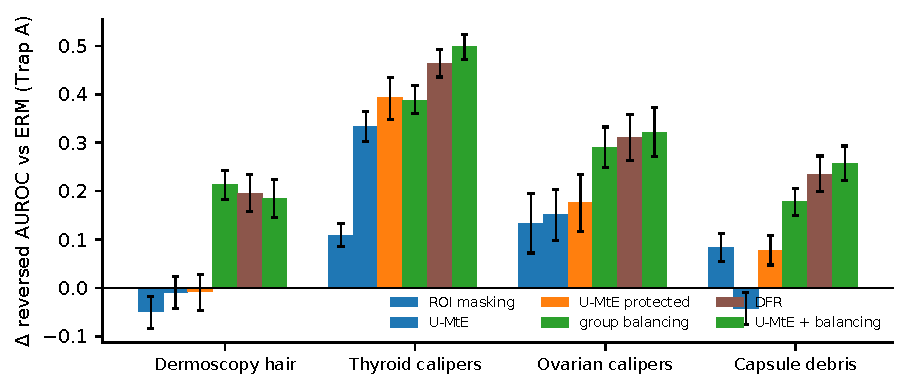
\includegraphics[width=0.9\linewidth]{../stage6_remedies_audit_paper/figures/remedies.pdf}
\caption{Remedies in the in-ROI trap (change in reversed AUROC versus ERM, DINOv2, crossed 95\% CIs).}\label{s6:fig:rem}\end{figure}
{\scriptsize
\begin{longtable}{p{3.4cm}p{4.2cm}p{3.5cm}p{3.5cm}}
\caption{Every remedy in every real-artifact trap and encoder: change in reversed-test AUROC versus ERM (5 seeds $\times$ 5 grouped folds, crossed CIs). U-MtE and the augmentation arm use only the ROI mask; balancing, DFR and their combinations need image-level artifact labels.}\label{s6:tab:remall}\\\toprule
Cohort, encoder & Arm $-$ ERM & Trap A (in ROI) & Trap B (outside) \\\midrule
\endfirsthead
\toprule Cohort, encoder & Arm $-$ ERM & Trap A (in ROI) & Trap B (outside) \\\midrule
\endhead
\bottomrule
\endlastfoot
Dermoscopy hair, DINOv2 & masking & $-0.049$ [$-0.083, -0.018$] & $+0.098$ [$+0.060, +0.136$] \\
 & U-MtE & $-0.009$ [$-0.043, +0.024$] & $+0.121$ [$+0.083, +0.160$] \\
 & U-MtE protected & $-0.008$ [$-0.046, +0.028$] & $+0.124$ [$+0.077, +0.170$] \\
 & same overlays as augmentation & $-0.044$ [$-0.078, -0.012$] & $+0.107$ [$+0.070, +0.145$] \\
 & group balancing & $+0.213$ [$+0.183, +0.243$] & $+0.204$ [$+0.166, +0.245$] \\
 & DFR & $+0.196$ [$+0.157, +0.235$] & $+0.196$ [$+0.147, +0.251$] \\
 & masking + DFR & $+0.152$ [$+0.103, +0.202$] & $+0.206$ [$+0.142, +0.267$] \\
 & U-MtE + balancing & $+0.185$ [$+0.145, +0.224$] & $+0.240$ [$+0.197, +0.283$] \\
Thyroid calipers, DINOv2 & masking & $+0.109$ [$+0.085, +0.133$] & $+0.348$ [$+0.307, +0.388$] \\
 & U-MtE & $+0.333$ [$+0.302, +0.364$] & $+0.347$ [$+0.308, +0.386$] \\
 & U-MtE protected & $+0.393$ [$+0.347, +0.434$] & $+0.349$ [$+0.310, +0.389$] \\
 & same overlays as augmentation & $+0.118$ [$+0.094, +0.143$] & $+0.345$ [$+0.305, +0.385$] \\
 & group balancing & $+0.388$ [$+0.360, +0.418$] & $+0.254$ [$+0.218, +0.292$] \\
 & DFR & $+0.463$ [$+0.436, +0.492$] & $+0.312$ [$+0.262, +0.362$] \\
 & masking + DFR & $+0.537$ [$+0.506, +0.567$] & $+0.357$ [$+0.313, +0.400$] \\
 & U-MtE + balancing & $+0.498$ [$+0.471, +0.524$] & $+0.371$ [$+0.329, +0.412$] \\
Thyroid calipers, MedSigLIP & masking & $+0.053$ [$+0.032, +0.073$] & $+0.248$ [$+0.200, +0.293$] \\
 & U-MtE & $+0.299$ [$+0.270, +0.328$] & $+0.276$ [$+0.232, +0.318$] \\
 & U-MtE protected & $+0.358$ [$+0.330, +0.388$] & $+0.271$ [$+0.224, +0.318$] \\
 & same overlays as augmentation & $+0.074$ [$+0.053, +0.095$] & $+0.248$ [$+0.202, +0.293$] \\
 & group balancing & $+0.409$ [$+0.382, +0.436$] & $+0.201$ [$+0.161, +0.241$] \\
 & DFR & $+0.463$ [$+0.437, +0.489$] & $+0.243$ [$+0.207, +0.282$] \\
 & masking + DFR & $+0.517$ [$+0.490, +0.545$] & $+0.279$ [$+0.234, +0.324$] \\
 & U-MtE + balancing & $+0.505$ [$+0.478, +0.531$] & $+0.313$ [$+0.269, +0.358$] \\
Thyroid calipers, ConvNeXt & masking & $-0.004$ [$-0.029, +0.020$] & $+0.271$ [$+0.228, +0.314$] \\
 & U-MtE & $+0.131$ [$+0.087, +0.171$] & $+0.276$ [$+0.231, +0.320$] \\
 & U-MtE protected & $+0.179$ [$+0.112, +0.236$] & $+0.286$ [$+0.241, +0.332$] \\
 & same overlays as augmentation & $+0.003$ [$-0.021, +0.027$] & $+0.270$ [$+0.227, +0.313$] \\
 & group balancing & $+0.326$ [$+0.305, +0.348$] & $+0.222$ [$+0.186, +0.258$] \\
 & DFR & $+0.369$ [$+0.335, +0.405$] & $+0.260$ [$+0.212, +0.305$] \\
 & masking + DFR & $+0.408$ [$+0.372, +0.442$] & $+0.307$ [$+0.259, +0.354$] \\
 & U-MtE + balancing & $+0.397$ [$+0.362, +0.434$] & $+0.313$ [$+0.266, +0.358$] \\
Ovarian calipers, DINOv2 & masking & $+0.132$ [$+0.072, +0.196$] & $+0.302$ [$+0.225, +0.378$] \\
 & U-MtE & $+0.152$ [$+0.098, +0.203$] & $+0.317$ [$+0.242, +0.388$] \\
 & U-MtE protected & $+0.175$ [$+0.116, +0.235$] & $+0.322$ [$+0.243, +0.398$] \\
 & same overlays as augmentation & $+0.117$ [$+0.054, +0.178$] & $+0.305$ [$+0.224, +0.383$] \\
 & group balancing & $+0.290$ [$+0.248, +0.332$] & $+0.256$ [$+0.190, +0.320$] \\
 & DFR & $+0.310$ [$+0.263, +0.357$] & $+0.278$ [$+0.209, +0.349$] \\
 & masking + DFR & $+0.339$ [$+0.284, +0.393$] & $+0.347$ [$+0.264, +0.428$] \\
 & U-MtE + balancing & $+0.321$ [$+0.271, +0.372$] & $+0.343$ [$+0.265, +0.419$] \\
Ovarian calipers, MedSigLIP & masking & $+0.002$ [$-0.048, +0.051$] & $+0.180$ [$+0.120, +0.238$] \\
 & U-MtE & $+0.212$ [$+0.163, +0.260$] & $+0.191$ [$+0.136, +0.245$] \\
 & U-MtE protected & $+0.155$ [$+0.098, +0.209$] & $+0.166$ [$+0.108, +0.224$] \\
 & same overlays as augmentation & $+0.018$ [$-0.027, +0.062$] & $+0.179$ [$+0.123, +0.235$] \\
 & group balancing & $+0.302$ [$+0.254, +0.351$] & $+0.149$ [$+0.103, +0.197$] \\
 & DFR & $+0.370$ [$+0.320, +0.420$] & $+0.210$ [$+0.154, +0.265$] \\
 & masking + DFR & $+0.356$ [$+0.299, +0.411$] & $+0.229$ [$+0.161, +0.296$] \\
 & U-MtE + balancing & $+0.364$ [$+0.312, +0.416$] & $+0.219$ [$+0.161, +0.277$] \\
Capsule debris, DINOv2 & masking & $+0.084$ [$+0.055, +0.112$] & $+0.461$ [$+0.415, +0.506$] \\
 & U-MtE & $-0.042$ [$-0.076, -0.009$] & $+0.441$ [$+0.396, +0.483$] \\
 & U-MtE protected & $+0.078$ [$+0.047, +0.107$] & $+0.442$ [$+0.397, +0.486$] \\
 & same overlays as augmentation & $+0.096$ [$+0.067, +0.126$] & $+0.462$ [$+0.417, +0.505$] \\
 & group balancing & $+0.179$ [$+0.150, +0.205$] & $+0.244$ [$+0.216, +0.272$] \\
 & DFR & $+0.234$ [$+0.199, +0.273$] & $+0.287$ [$+0.239, +0.335$] \\
 & masking + DFR & $+0.312$ [$+0.275, +0.349$] & $+0.446$ [$+0.393, +0.497$] \\
 & U-MtE + balancing & $+0.258$ [$+0.221, +0.293$] & $+0.471$ [$+0.428, +0.514$] \\
Capsule debris, MedSigLIP & masking & $+0.117$ [$+0.088, +0.147$] & $+0.452$ [$+0.407, +0.495$] \\
 & U-MtE & $-0.113$ [$-0.146, -0.080$] & $+0.406$ [$+0.362, +0.450$] \\
 & U-MtE protected & $+0.088$ [$+0.055, +0.121$] & $+0.448$ [$+0.404, +0.491$] \\
 & same overlays as augmentation & $+0.136$ [$+0.106, +0.166$] & $+0.451$ [$+0.407, +0.495$] \\
 & group balancing & $+0.225$ [$+0.203, +0.248$] & $+0.240$ [$+0.211, +0.269$] \\
 & DFR & $+0.254$ [$+0.222, +0.286$] & $+0.279$ [$+0.242, +0.320$] \\
 & masking + DFR & $+0.345$ [$+0.312, +0.378$] & $+0.438$ [$+0.391, +0.483$] \\
 & U-MtE + balancing & $+0.269$ [$+0.232, +0.308$] & $+0.453$ [$+0.410, +0.496$] \\
Capsule debris, ConvNeXt & masking & $+0.084$ [$+0.049, +0.118$] & $+0.403$ [$+0.358, +0.448$] \\
 & U-MtE & $+0.009$ [$-0.024, +0.040$] & $+0.378$ [$+0.334, +0.422$] \\
 & U-MtE protected & $+0.108$ [$+0.074, +0.142$] & $+0.383$ [$+0.337, +0.429$] \\
 & same overlays as augmentation & $+0.099$ [$+0.066, +0.131$] & $+0.406$ [$+0.361, +0.449$] \\
 & group balancing & $+0.197$ [$+0.172, +0.221$] & $+0.226$ [$+0.198, +0.256$] \\
 & DFR & $+0.255$ [$+0.223, +0.291$] & $+0.293$ [$+0.234, +0.346$] \\
 & masking + DFR & $+0.330$ [$+0.296, +0.364$] & $+0.453$ [$+0.403, +0.502$] \\
 & U-MtE + balancing & $+0.273$ [$+0.231, +0.312$] & $+0.433$ [$+0.384, +0.480$] \\
\end{longtable}}


\subsubsection{Which model is most robust?}
A reversed-test gain can come from inverting the shortcut rather than removing it. Table~\ref{s6:tab:rob} therefore reports
$\min$(reversed, correlated) AUROC. With image-level artifact labels, U-MtE with balancing is the most robust model for
thyroid with all three encoders (e.g.\ \sSixRobThyroidDINOvTwomtebalanced{} with DINOv2) and for the ovary with MedSigLIP
(\sSixRobOvarianMedSigLIPmtebalanced); masking with DFR is best for capsule (\sSixRobCapsuleDINOvTwomaskdfr) and the DINOv2
ovary (\sSixRobOvarianDINOvTwomaskdfr); plain balancing for hair (\sSixRobDermoscopyDINOvTwobalanced) and DFR for chest
drains (\sSixRobChestRADDINOdfr). DFR and masking + DFR over-correct on thyroid: their correlated AUROC falls below the
reversed one (marked $^\dagger$). Without artifact labels, protected U-MtE is the most robust label-free arm for thyroid; for
capsule the best label-free choice is U-MtE combined with JTT (Table~\ref{s6:tab:jtt}).
\begin{table}[H]\centering\scriptsize
\caption{Robustness summary in the in-ROI trap: $\min$(reversed, correlated) AUROC per arm (mean over seeds; best per row in bold; $^\dagger$ = the arm flips the shortcut, correlated $<$ reversed $-0.02$).}\label{s6:tab:rob}
\resizebox{\linewidth}{!}{\begin{tabular}{lcccccccccc}\toprule
Trap A & ERM & mask & U-MtE & U-MtE prot. & overlay aug. & JTT & balanced & DFR & mask+DFR & U-MtE+bal. \\\midrule
Dermoscopy hair, DINOv2 & 0.510 & 0.460 & 0.500 & 0.502 & 0.466 & 0.575 & \textbf{0.722} & 0.705 & 0.662 & 0.695 \\
Thyroid calipers, DINOv2 & 0.289 & 0.398 & 0.622 & 0.682 & 0.407 & 0.417 & 0.677 & 0.669$^\dagger$ & 0.751$^\dagger$ & \textbf{0.787} \\
Thyroid calipers, MedSigLIP & 0.289 & 0.341 & 0.587 & 0.647 & 0.362 & -- & 0.698 & 0.722$^\dagger$ & 0.772$^\dagger$ & \textbf{0.793} \\
Thyroid calipers, ConvNeXt & 0.357 & 0.353 & 0.488 & 0.536 & 0.361 & -- & 0.684 & 0.669$^\dagger$ & 0.713$^\dagger$ & \textbf{0.755} \\
Ovarian calipers, DINOv2 & 0.413 & 0.545 & 0.565 & 0.588 & 0.530 & 0.440 & 0.703 & 0.689$^\dagger$ & \textbf{0.752} & 0.734 \\
Ovarian calipers, MedSigLIP & 0.426 & 0.428 & 0.638 & 0.581 & 0.444 & -- & 0.729 & 0.756$^\dagger$ & 0.782 & \textbf{0.790} \\
Capsule debris, DINOv2 & 0.581 & 0.665 & 0.539 & 0.659 & 0.678 & 0.596 & 0.760 & 0.816 & \textbf{0.892} & 0.839 \\
Capsule debris, MedSigLIP & 0.570 & 0.687 & 0.457 & 0.658 & 0.706 & -- & 0.796 & 0.825 & \textbf{0.915} & 0.839 \\
Capsule debris, ConvNeXt & 0.528 & 0.612 & 0.537 & 0.636 & 0.627 & -- & 0.725 & 0.783 & \textbf{0.858} & 0.801 \\
Chest drains, RAD-DINO & 0.194 & 0.232 & 0.272 & 0.275 & 0.236 & 0.179 & 0.540 & \textbf{0.666} & 0.635 & 0.461 \\
\bottomrule\end{tabular}}
\end{table}


\subsubsection{The 16-test primary family}
Table~\ref{s6:tab:primall}. The four location tests (P1) and twelve remedy tests --- protected U-MtE $>$ mask (P2), erase $>$
augment with the same overlays (P3), U-MtE+balancing $>$ balancing (P4), in each of the four cohorts --- were grouped
into one Holm family after the individual results were known (conservative bookkeeping, not a pre-registered family).
\sSixNPrimOK{} of \sSixNPrim{} are supported: all four P1; P2 in hair, thyroid and ovary (not capsule); P3 in hair and
thyroid (capsule significant in the opposite direction; ovary not after Holm); P4 in thyroid and capsule.
\begin{table}[H]\centering\scriptsize
\caption{The 16-test primary family (DINOv2, Trap~A reversed test unless stated): the four location tests and the twelve remedy tests, Holm-corrected together.}\label{s6:tab:primall}
\resizebox{\linewidth}{!}{\begin{tabular}{lccccc}\toprule
Family & Cohort & Estimate [95\% CI] & $p$ & $p$ (Holm, 16) & Supported \\\midrule
P1 location crossover & ISIC hair (DINOv2) & $+0.147$ [$+0.111, +0.185$] & 0.0001 & 0.0016 & \ok \\
P1 location crossover & Thyroid (DINOv2) & $+0.239$ [$+0.196, +0.280$] & 0.0001 & 0.0016 & \ok \\
P1 location crossover & Capsule (DINOv2) & $+0.377$ [$+0.327, +0.426$] & 0.0001 & 0.0016 & \ok \\
P1 location crossover & Ovary (DINOv2) & $+0.170$ [$+0.087, +0.252$] & 0.0001 & 0.0016 & \ok \\
P2 U-MtE (protected) > mask & ISIC hair & $+0.042$ [$+0.024, +0.058$] & 0.0001 & 0.0016 & \ok \\
P2 U-MtE (protected) > mask & Thyroid & $+0.283$ [$+0.237, +0.329$] & 0.0001 & 0.0016 & \ok \\
P2 U-MtE (protected) > mask & Capsule & $-0.006$ [$-0.018, +0.006$] & 0.2946 & 0.3486 & \no \\
P2 U-MtE (protected) > mask & Ovary & $+0.043$ [$+0.023, +0.065$] & 0.0001 & 0.0016 & \ok \\
P3 erase > augment & ISIC hair & $+0.035$ [$+0.017, +0.055$] & 0.0002 & 0.0016 & \ok \\
P3 erase > augment & Thyroid & $+0.215$ [$+0.189, +0.244$] & 0.0001 & 0.0016 & \ok \\
P3 erase > augment & Capsule & $-0.139$ [$-0.158, -0.120$] & 0.0001 & 0.0016 & \no{} (opposite) \\
P3 erase > augment & Ovary & $+0.035$ [$+0.003, +0.067$] & 0.0326 & 0.1304 & \no \\
P4 U-MtE+balanced > balanced & ISIC hair & $-0.028$ [$-0.064, +0.007$] & 0.1162 & 0.3486 & \no \\
P4 U-MtE+balanced > balanced & Thyroid & $+0.110$ [$+0.079, +0.142$] & 0.0001 & 0.0016 & \ok \\
P4 U-MtE+balanced > balanced & Capsule & $+0.079$ [$+0.042, +0.115$] & 0.0002 & 0.0016 & \ok \\
P4 U-MtE+balanced > balanced & Ovary & $+0.031$ [$-0.014, +0.077$] & 0.1730 & 0.3486 & \no \\
\bottomrule\end{tabular}}
\end{table}


\subsubsection{Remedies in the controlled sweeps}
Tables~\ref{s6:tab:swrem} and~\ref{s6:tab:swisic}. With DINOv2 and RAD-DINO, U-MtE beats masking at full overlap in every modality sweep
(thyroid \sSixSwthyroiddinoFiveOneEightUmte, capsule \sSixSwcapsuledinoFiveOneEightUmte, chest tube
\sSixSwcxrraddinoFiveOneEightUmte).
With MedSigLIP it fails on both the synthetic caliper and the synthetic debris; protection turns the debris failure into
a gain (\sSixSwcapsulemedsiglipProt) but not the caliper failure (\sSixSwthyroidmedsiglipProt). U-MtE with balancing beats
masking in every sweep and has no positive location interaction (dermoscopy: \sSixSwIsicBalInter, against masking's large
positive one). On the dermoscopy ruler, the insert-then-erase precursor on unmasked features helps
(\sSixSwIsicUitwoe) while plain U-MtE does not (\sSixSwIsicUmte): with the
synthetic ruler, the subspace estimated from generic overlays evidently misses the direction of the retained ruler, and
only the balanced variant repairs it.
\begin{table}[H]\centering\scriptsize
\caption{Remedies in the controlled sweeps at full overlap (reversed-test AUROC, crossed CIs).}\label{s6:tab:swrem}
\resizebox{\linewidth}{!}{\begin{tabular}{lcccc}\toprule
Controlled sweep, $r=1$ & U-MtE $-$ mask & U-MtE protected $-$ mask & U-MtE+bal.\ $-$ mask & U-MtE+bal.\ $-$ balanced \\\midrule
Thyroid caliper, DINOv2 & $+0.278$ [$+0.214, +0.344$] & $+0.287$ [$+0.141, +0.464$] & $+0.470$ [$+0.391, +0.550$] & $+0.091$ [$+0.013, +0.172$] \\
Thyroid caliper, MedSigLIP & $-0.076$ [$-0.120, -0.034$] & $-0.041$ [$-0.095, +0.002$] & $+0.458$ [$+0.393, +0.525$] & $+0.069$ [$+0.002, +0.136$] \\
Ovarian caliper, DINOv2 & $+0.140$ [$+0.061, +0.225$] & $+0.114$ [$+0.043, +0.192$] & $+0.251$ [$+0.157, +0.355$] & $-0.032$ [$-0.165, +0.104$] \\
Capsule debris, DINOv2 & $+0.121$ [$+0.078, +0.170$] & $+0.130$ [$+0.083, +0.189$] & $+0.211$ [$+0.134, +0.297$] & $+0.057$ [$-0.008, +0.121$] \\
Capsule debris, MedSigLIP & $-0.190$ [$-0.265, -0.120$] & $+0.114$ [$+0.022, +0.238$] & $+0.299$ [$+0.195, +0.398$] & $-0.018$ [$-0.101, +0.065$] \\
Chest tube, RAD-DINO & $+0.134$ [$+0.113, +0.156$] & $+0.144$ [$+0.125, +0.164$] & $+0.168$ [$+0.145, +0.191$] & $-0.031$ [$-0.042, -0.021$] \\
\bottomrule\end{tabular}}
\end{table}

\begin{table}[H]\centering\scriptsize
\caption{The dermoscopy ruler sweep at full overlap: the insert-then-erase precursor (U-I2E, erasing on unmasked features) and the mask-then-erase variants, versus ERM (crossed CIs).}\label{s6:tab:swisic}
\resizebox{\linewidth}{!}{\begin{tabular}{lcccc}\toprule
Dermoscopy ruler sweep, $r=1$ (DINOv2) & U-I2E $-$ ERM & U-MtE $-$ ERM & U-MtE protected $-$ ERM & U-MtE+bal.\ $-$ ERM \\\midrule
change in reversed AUROC & $+0.197$ [$+0.146, +0.247$] & $-0.007$ [$-0.085, +0.070$] & $+0.091$ [$-0.016, +0.185$] & $+0.243$ [$+0.167, +0.317$] \\
\bottomrule\end{tabular}}
\end{table}


\subsubsection{Erasure versus augmentation, protection, and other contrasts}
Table~\ref{s6:tab:supp}. The \emph{same} overlays used as training augmentation instead of for erasure gain almost nothing
over masking (Table~\ref{s6:tab:remall}, ``same overlays as augmentation''), while erasure gains \sSixScthyroidMedSigLIPmtemteaug{}
over augmentation with MedSigLIP and \sSixScthyroidConvNeXtmtemteaug{} with ConvNeXt on thyroid: it is the subspace
estimation, not exposure to overlays, that helps. Protection is a safety net: it costs nothing on hair
(\sSixSchairmteprotectmte), helps thyroid (\sSixScthyroidmteprotectmte) and removes the capsule failure (protected
$-$ mask \sSixSccapsulemteprotectmask{} versus unprotected \sSixSccapsulemtemask).
\begin{table}[H]\centering\scriptsize
\caption{Secondary remedy contrasts (reversed test, crossed CIs).}\label{s6:tab:supp}
\begin{tabular}{lcc}\toprule
Cohort & Contrast (Trap A) & Estimate [95\% CI] \\\midrule
hair & mte $-$ mask & $+0.040$ [$+0.024, +0.056$] \\
hair & mte\_protect $-$ mte & $+0.001$ [$-0.016, +0.017$] \\
thyroid & mte\_protect $-$ mte & $+0.059$ [$+0.019, +0.096$] \\
thyroid & mte $-$ jtt & $+0.206$ [$+0.171, +0.241$] \\
ovary & mte $-$ jtt & $+0.125$ [$+0.063, +0.189$] \\
thyroid MedSigLIP & mte $-$ mte\_aug & $+0.225$ [$+0.202, +0.247$] \\
thyroid ConvNeXt & mte $-$ mte\_aug & $+0.128$ [$+0.093, +0.161$] \\
thyroid ConvNeXt & mte $-$ mask & $+0.135$ [$+0.102, +0.168$] \\
capsule & mte $-$ mask & $-0.126$ [$-0.146, -0.107$] \\
capsule & mte\_protect $-$ mask & $-0.006$ [$-0.018, +0.006$] \\
\bottomrule\end{tabular}
\end{table}


\subsubsection{How many directions must be erased?}
Table~\ref{s6:tab:rank}. On thyroid the gain is robust for every setting that erases $\ge16$ directions or $\ge50\%$ of the
overlay-shift energy; one to four directions recover only a third of it --- the overlay shift is multi-dimensional. In these
cohorts the 90\% rule reaches the cap of 64 directions. Unprotected erasure harms capsule more the more directions it
removes, as the theory's $\rho$ predicts; the protected variant never harms capsule and helps the ovary at every rank.
\begin{table}[H]\centering\scriptsize
\caption{Erasure-rank ablation (DINOv2, Trap A): reversed-AUROC difference to masking (mean over seeds) for the energy rule (share of held-out overlay-shift energy removed; cap 64) and for fixed ranks $k$.}\label{s6:tab:rank}
\begin{tabular}{lccccc}\toprule
Erased rank & Thyroid U-MtE & Ovary U-MtE & Ovary protected & Capsule U-MtE & Capsule protected \\\midrule
energy 0.50 & $+0.190$ & $-0.003$ & $+0.033$ & $-0.067$ & $-0.006$ \\
energy 0.90 (main) & $+0.224$ & $+0.020$ & $+0.043$ & $-0.126$ & $-0.006$ \\
energy 0.99 & $+0.224$ & $+0.020$ & $+0.043$ & $-0.126$ & $-0.006$ \\
$k=1$ & $+0.068$ & $+0.010$ & $+0.009$ & $+0.001$ & $+0.000$ \\
$k=4$ & $+0.056$ & $-0.038$ & $+0.015$ & $-0.010$ & $-0.003$ \\
$k=16$ & $+0.183$ & $-0.011$ & $+0.020$ & $-0.058$ & $-0.009$ \\
$k=64$ & $+0.224$ & $+0.020$ & $+0.043$ & $-0.126$ & $-0.006$ \\
\bottomrule\end{tabular}
\end{table}


\subsubsection{Encoder size}
Table~\ref{s6:tab:scalerem}. Protected U-MtE beats masking in thyroid and ovary at every DINOv2 size; on capsule protection
is less complete with ViT-L.
\begin{table}[H]\centering\scriptsize
\caption{U-MtE across encoder sizes (crossed CIs).}\label{s6:tab:scalerem}
\begin{tabular}{lccc}\toprule
Cohort & DINOv2 & U-MtE $-$ mask (Trap A) & U-MtE protected $-$ mask \\\midrule
Thyroid & ViT-S/14 & $+0.192$ [$+0.159, +0.227$] & $+0.225$ [$+0.168, +0.276$] \\
Thyroid & ViT-B/14 & $+0.224$ [$+0.195, +0.254$] & $+0.283$ [$+0.237, +0.329$] \\
Thyroid & ViT-L/14 & $+0.246$ [$+0.216, +0.279$] & $+0.274$ [$+0.243, +0.306$] \\
Ovary & ViT-S/14 & $+0.121$ [$+0.084, +0.158$] & $+0.103$ [$+0.074, +0.134$] \\
Ovary & ViT-B/14 & $+0.020$ [$-0.016, +0.054$] & $+0.043$ [$+0.023, +0.065$] \\
Ovary & ViT-L/14 & $+0.094$ [$+0.061, +0.127$] & $+0.060$ [$+0.037, +0.084$] \\
Capsule & ViT-S/14 & $-0.153$ [$-0.172, -0.134$] & $-0.002$ [$-0.018, +0.016$] \\
Capsule & ViT-B/14 & $-0.126$ [$-0.146, -0.107$] & $-0.006$ [$-0.018, +0.006$] \\
Capsule & ViT-L/14 & $-0.097$ [$-0.114, -0.079$] & $-0.044$ [$-0.056, -0.032$] \\
\bottomrule\end{tabular}
\end{table}


\subsubsection{Published baselines and alternatives}
Table~\ref{s6:tab:jtt} (crossed intervals), Table~\ref{s6:tab:regen} (analyses first archived without per-image predictions and
regenerated with them; crossed intervals) and Table~\ref{s6:tab:archived} (point estimates of analyses whose predictions were
not saved).
\begin{itemize}[leftmargin=*]\itemsep1pt
\item \textbf{JTT} (label-free): U-MtE beats it on thyroid (\sSixScthyroidmtejtt) and ovary (\sSixScovarymtejtt); JTT wins
on hair ($\min$(rev, corr) \sSixBlDermoscopyjtt{} versus \sSixBlDermoscopymte); on capsule U-MtE+JTT is the most robust
label-free combination (\sSixBlCapsuleumtejtt).
\item \textbf{SPLINCE} (needs artifact labels): the faithful implementation removes much disease signal (clean AUROC
\sSixBlCleanThyroidsplice{} on thyroid) and still inverts the shortcut on capsule; U-MtE with balancing is more robust
on thyroid, capsule and hair (\sSixBlThyroidmtebalanced{} versus \sSixBlThyroidsplice; \sSixBlCapsulemtebalanced{} versus
\sSixBlCapsulesplice; \sSixBlDermoscopymtebalanced{} versus \sSixBlDermoscopysplice).
\item \textbf{LaMa inpainting} of the detected artifact pixels, followed by masking, is a strong baseline that needs artifact
masks (over masking: thyroid \sSixRgLaMamaskingthyroidmasklamamask, ovary \sSixRgLaMamaskingovarymasklamamask). Protected
U-MtE, which needs no artifact mask, exceeds it on thyroid (\sSixRgLaMamaskingthyroidmteprotectmasklama) and is below it on
ovary (\sSixRgLaMamaskingovarymteprotectmasklama) and hair (\sSixArLaMaisicmteprotectmasklama, archived point estimate);
U-MtE with balancing beats it everywhere. The thyroid comparison changed when the run was regenerated (archived
$-0.009$): the protected arm reproduced about 0.06 higher than in its first run, with unchanged code for that arm, and
now agrees with the protected arm of the main regenerated run (\texttt{results/bootstrap\_correction/archived\_old\_vs\_new.md}).
\item \textbf{Text-prompted erasure} with MedSigLIP and DermLIP is a near no-op ($\le$ \sSixArtextpromptedovarymasktexterasemask{}
over masking): the text-space artifact direction does not coincide with the image-space direction along which the artifact
moves the representation.
\item \textbf{SLAS} localises hair from a few annotated images, but the gain it enables is capped by what hair pixels carry:
removing \emph{every} real hair patch (an oracle) gains only \sSixArSLAShairmtsoracletokmask{} over token-level masking.
\item \textbf{Pseudo-group balancing} from an overlay detector helps on thyroid (reversed \sSixArpseudogroupthyroidumtepbalreversedAUROC{}
versus \sSixArpseudogroupthyroidmtereversedAUROC{} for U-MtE) and not on hair, where the detector cannot see hair.
\item \textbf{Erasure + DFR} adds at most about 0.01 over masking + DFR: once a group-robust head is used, masking does the rest.
\item \textbf{Validation-driven selectors} beat masking in every cohort and are within about 0.02 of the best candidate, but
neither is uniformly best; admitting DFR as a candidate fixes chest drains and makes the choice noisier elsewhere.
\item \textbf{Chest drains}: U-MtE gains \sSixRgchestRADDINOdrainsmtemask{} over masking with RAD-DINO and nothing with
DINOv2 (\sSixRgchestDINOvTwodrainsmtemask); DFR is best.
\item \textbf{Templates instead of generic overlays} on capsule debris make erasure worse
(\sSixRgUMtEtemplatescapsulemtemask{} against masking); disease protection removes that failure
(\sSixRgUMtEtemplatescapsulemteprotectmask).
\end{itemize}
{\scriptsize
\begin{longtable}{lccccc}
\caption{Published baselines: JTT (label-free error upweighting) and SPLINCE (faithful whitened implementation of the covariance-preserving concept projection, needs artifact labels), beside U-MtE (mean over seeds).}\label{s6:tab:jtt}\\\toprule
Cohort (Trap A) & Arm & clean & correlated & reversed & min(rev, corr) \\\midrule
\endfirsthead
\toprule Cohort (Trap A) & Arm & clean & correlated & reversed & min(rev, corr) \\\midrule
\endhead
\bottomrule
\endlastfoot
Thyroid & JTT & 0.629 & 0.829 & 0.417 & 0.417 \\
Thyroid & mask & 0.689 & 0.908 & 0.398 & 0.398 \\
Thyroid & mask+JTT & 0.699 & 0.888 & 0.455 & 0.455 \\
Thyroid & U-MtE & 0.729 & 0.824 & 0.622 & 0.622 \\
Thyroid & U-MtE+JTT & 0.629 & 0.848 & 0.363 & 0.363 \\
Thyroid & balanced & 0.717 & 0.757 & 0.677 & 0.677 \\
Thyroid & mask+SPLINCE & 0.603 & 0.599 & 0.610 & 0.599 \\
Thyroid & U-MtE+bal. & 0.798 & 0.804 & 0.787 & 0.787 \\
Thyroid & U-MtE prot. & 0.728 & 0.769 & 0.682 & 0.682 \\
Thyroid & SPLINCE & 0.577 & 0.565 & 0.587 & 0.565 \\
Capsule & JTT & 0.786 & 0.928 & 0.596 & 0.596 \\
Capsule & mask & 0.860 & 0.972 & 0.665 & 0.665 \\
Capsule & mask+JTT & 0.878 & 0.956 & 0.760 & 0.760 \\
Capsule & U-MtE & 0.815 & 0.972 & 0.539 & 0.539 \\
Capsule & U-MtE+JTT & 0.881 & 0.945 & 0.787 & 0.787 \\
Capsule & balanced & 0.847 & 0.916 & 0.760 & 0.760 \\
Capsule & mask+SPLINCE & 0.786 & 0.715 & 0.852 & 0.715 \\
Capsule & U-MtE+bal. & 0.899 & 0.939 & 0.839 & 0.839 \\
Capsule & U-MtE prot. & 0.855 & 0.970 & 0.659 & 0.659 \\
Capsule & SPLINCE & 0.741 & 0.668 & 0.788 & 0.668 \\
Dermoscopy hair & JTT & 0.745 & 0.898 & 0.564 & 0.564 \\
Dermoscopy hair & mask & 0.712 & 0.916 & 0.454 & 0.454 \\
Dermoscopy hair & mask+JTT & 0.711 & 0.880 & 0.509 & 0.509 \\
Dermoscopy hair & U-MtE & 0.735 & 0.913 & 0.506 & 0.506 \\
Dermoscopy hair & U-MtE+JTT & 0.729 & 0.885 & 0.541 & 0.541 \\
Dermoscopy hair & balanced & 0.785 & 0.850 & 0.722 & 0.722 \\
Dermoscopy hair & mask+SPLINCE & 0.598 & 0.572 & 0.621 & 0.572 \\
Dermoscopy hair & U-MtE+bal. & 0.778 & 0.860 & 0.695 & 0.695 \\
Dermoscopy hair & U-MtE prot. & 0.718 & 0.904 & 0.502 & 0.502 \\
Dermoscopy hair & SPLINCE & 0.600 & 0.575 & 0.637 & 0.575 \\
\end{longtable}}

\begin{table}[H]\centering\scriptsize
\caption{Remedy analyses regenerated with per-image predictions after the other runs (same commands and seeds; crossed bootstrap).}\label{s6:tab:regen}
\begin{tabular}{p{4.0cm}p{2.0cm}p{4.4cm}c}\toprule
Analysis & Cohort & Contrast (Trap A, reversed) & Estimate [95\% CI] \\\midrule
LaMa inpainting then masking & thyroid & mask\_lama $-$ mask & $+0.224$ [$+0.206, +0.242$] \\
 & thyroid & mte\_protect $-$ mask\_lama & $+0.060$ [$+0.013, +0.105$] \\
 & thyroid & mte\_balanced $-$ mask\_lama & $+0.165$ [$+0.146, +0.185$] \\
 & ovary & mask\_lama $-$ mask & $+0.128$ [$+0.084, +0.169$] \\
 & ovary & mte\_protect $-$ mask\_lama & $-0.085$ [$-0.120, -0.050$] \\
 & ovary & mte\_balanced $-$ mask\_lama & $+0.061$ [$+0.026, +0.095$] \\
U-MtE from real-debris templates & capsule & mte $-$ mask & $-0.392$ [$-0.425, -0.360$] \\
 & capsule & mte\_protect $-$ mask & $+0.003$ [$-0.014, +0.021$] \\
chest drains, RAD-DINO & drains & mte $-$ mask & $+0.040$ [$+0.023, +0.057$] \\
 & drains & mte\_protect $-$ mask & $+0.042$ [$+0.028, +0.058$] \\
 & drains & mte $-$ jtt & $+0.094$ [$+0.077, +0.111$] \\
 & drains & mte\_balanced $-$ balanced & $-0.079$ [$-0.106, -0.044$] \\
chest drains, DINOv2 & drains & mte $-$ mask & $-0.001$ [$-0.009, +0.008$] \\
 & drains & mte\_protect $-$ mask & $-0.003$ [$-0.013, +0.006$] \\
 & drains & mte $-$ jtt & $-0.005$ [$-0.021, +0.011$] \\
 & drains & mte\_balanced $-$ balanced & $+0.031$ [$-0.023, +0.079$] \\
\bottomrule\end{tabular}
\end{table}

{\scriptsize
\begin{longtable}{p{4.0cm}p{3.6cm}p{5.2cm}c}
\caption{Remedy analyses whose per-image predictions were not saved, so their intervals could not be re-estimated with the crossed bootstrap: \textbf{point estimates only}.}\label{s6:tab:archived}\\\toprule
Analysis & Cohort / run & Contrast (Trap A, reversed) & Point estimate \\\midrule
\endfirsthead
\toprule Analysis & Cohort / run & Contrast (Trap A, reversed) & Point estimate \\\midrule
\endhead
\bottomrule
\endlastfoot
LaMa inpainting (oracle masks) & isic & lama $-$ mask & $+0.145$ \\
 & isic & mask\_lama $-$ mask & $+0.127$ \\
 & isic & mte\_protect $-$ mask\_lama & $-0.086$ \\
 & isic & mte\_balanced $-$ mask\_lama & $+0.123$ \\
 & isic & lama $-$ erm & $+0.107$ \\
text-prompted erasure & thyroid & mask\_text\_erase $-$ mask & $+0.005$ \\
 & thyroid & mte $-$ mask & $+0.204$ \\
 & thyroid & mask\_text\_erase\_balanced $-$ balanced & $+0.056$ \\
 & ovary & mask\_text\_erase $-$ mask & $+0.008$ \\
 & ovary & mte $-$ mask & $+0.215$ \\
 & ovary & mask\_text\_erase\_balanced $-$ balanced & $-0.010$ \\
 & capsule & mask\_text\_erase $-$ mask & $+0.001$ \\
 & capsule & mte $-$ mask & $-0.236$ \\
 & capsule & mask\_text\_erase\_balanced $-$ balanced & $+0.066$ \\
 & hair (DermLIP) & mask\_text\_erase $-$ mask & $+0.004$ \\
 & hair (DermLIP) & mte $-$ mask & $-0.076$ \\
 & hair (DermLIP) & mask\_text\_erase\_balanced $-$ balanced & $-0.112$ \\
SLAS & hair & tok\_mask $-$ tok\_erm & $+0.030$ \\
 & hair & mts $-$ tok\_mask & $+0.022$ \\
 & hair & slas $-$ tok\_erm & $+0.008$ \\
 & hair & mts\_oracle $-$ tok\_mask & $+0.015$ \\
 & hair & mts\_balanced $-$ tok\_balanced & $+0.051$ \\
 & thyroid & tok\_mask $-$ tok\_erm & $+0.059$ \\
 & thyroid & mts $-$ tok\_mask & $+0.081$ \\
 & thyroid & slas $-$ tok\_erm & $+0.007$ \\
 & thyroid & mts\_oracle $-$ tok\_mask & $+0.047$ \\
 & thyroid & mts\_balanced $-$ tok\_balanced & $+0.070$ \\
erasure + DFR (U10) & thyroid & mte\_dfr $-$ dfr & $+0.101$ \\
 & thyroid & mte\_dfr $-$ mask\_dfr & $+0.007$ \\
 & thyroid & mask\_dfr $-$ dfr & $+0.095$ \\
 & capsule & mte\_dfr $-$ dfr & $+0.080$ \\
 & capsule & mte\_dfr $-$ mask\_dfr & $+0.000$ \\
 & capsule & mask\_dfr $-$ dfr & $+0.080$ \\
 & hair & mte\_dfr $-$ dfr & $-0.039$ \\
 & hair & mte\_dfr $-$ mask\_dfr & $+0.014$ \\
 & hair & mask\_dfr $-$ dfr & $-0.053$ \\
pseudo-group balancing (U8) & thyroid & umte\_pbal reversed AUROC & 0.663 \\
 & thyroid & mte reversed AUROC & 0.622 \\
 & thyroid & pbal reversed AUROC & 0.409 \\
 & thyroid & erm reversed AUROC & 0.289 \\
 & hair & umte\_pbal reversed AUROC & 0.510 \\
 & hair & mte reversed AUROC & 0.506 \\
 & hair & pbal reversed AUROC & 0.498 \\
 & hair & erm reversed AUROC & 0.491 \\
location-adaptive selection (U13) & thyroid & auto $-$ mask & $+0.395$ \\
 & thyroid & auto $-$ dfr & $+0.057$ \\
 & capsule & auto $-$ mask & $+0.168$ \\
 & capsule & auto $-$ dfr & $+0.047$ \\
 & hair & auto $-$ mask & $+0.251$ \\
 & hair & auto $-$ dfr & $-0.038$ \\
 & chest drains & auto $-$ mask & $+0.299$ \\
 & chest drains & auto $-$ dfr & $-0.144$ \\
split-validation selection (U14) & thyroid & auto $-$ mask & $+0.398$ \\
 & thyroid & auto $-$ dfr & $+0.060$ \\
 & capsule & auto $-$ mask & $+0.187$ \\
 & capsule & auto $-$ dfr & $+0.066$ \\
 & ovary & auto $-$ mask & $+0.170$ \\
 & ovary & auto $-$ dfr & $-0.007$ \\
 & hair & auto $-$ mask & $+0.234$ \\
 & hair & auto $-$ dfr & $-0.055$ \\
 & chest drains & auto $-$ mask & $+0.417$ \\
 & chest drains & auto $-$ dfr & $-0.026$ \\
\end{longtable}}


\subsubsection{Robustness of the remedy tests to leakage groups}
Table~\ref{s6:tab:embrem}. With the stricter embedding-based groups of Stage~4, the thyroid remedy tests are unchanged; in the
ovary, erase $>$ augment (P3) and U-MtE+balancing $>$ balancing (P4) lose significance: ``erase beats augment'' is robust in
thyroid and hair but fragile in the ovary.
\begin{table}[H]\centering\scriptsize
\caption{The remedy tests re-run with the stricter embedding-based leakage groups (cohorts without patient identifiers).}\label{s6:tab:embrem}
\begin{tabular}{lccc}\toprule
Cohort & Test & With embedding-based leakage groups & CI $>0$ \\\midrule
Thyroid & P2 U-MtE (protected) > mask & $+0.251$ [$+0.215, +0.284$] & yes \\
Thyroid & P3 erase > augment & $+0.192$ [$+0.160, +0.223$] & yes \\
Thyroid & P4 U-MtE+balanced > balanced & $+0.152$ [$+0.127, +0.177$] & yes \\
Ovary & P2 U-MtE (protected) > mask & $+0.051$ [$+0.020, +0.079$] & yes \\
Ovary & P3 erase > augment & $+0.024$ [$-0.014, +0.062$] & \textbf{no} \\
Ovary & P4 U-MtE+balanced > balanced & $+0.038$ [$-0.005, +0.081$] & \textbf{no} \\
Capsule & P2 U-MtE (protected) > mask & $-0.006$ [$-0.022, +0.014$] & \textbf{no} \\
Capsule & P3 erase > augment & $-0.128$ [$-0.158, -0.098$] & \textbf{no} \\
Capsule & P4 U-MtE+balanced > balanced & $+0.101$ [$+0.071, +0.132$] & yes \\
\bottomrule\end{tabular}
\end{table}


\subsubsection{Fully fine-tuned networks}
Table~\ref{s6:tab:ftrem}. Applying U-MtE \emph{after} fine-tuning does nothing (\sSixFtThyroidResNetFiveZeroMtePost): unconstrained
fine-tuning builds a task-specific caliper feature that generic overlays do not move. Remedies must act \emph{during} training.
Each component alone works for only one architecture on thyroid (invariance for ResNet-50, \sSixFtThyroidResNetFiveZeroMteFt;
prediction consistency for ViT-S, \sSixFtThyroidViTSOneSixConsFt). Combining projection, invariance and consistency
(\texttt{umte\_cons\_ft}, registered before it was run) improves on fine-tuned masking for both: ResNet-50
\sSixFtThyroidResNetFiveZeroUmteConsFt, ViT-S \sSixFtThyroidViTSOneSixUmteConsFt{} --- without any artifact annotation. It fails
on capsule (\sSixFtCapsuleResNetFiveZeroUmteConsFt), the pathology-like regime, and is not significant on the ovary
(\sSixFtOvaryResNetFiveZeroUmteConsFt{} with 15 clusters), where the fine-tuned network barely learns the task.
\begin{table}[H]\centering\scriptsize
\caption{Remedies for end-to-end fine-tuned networks: change in reversed-test AUROC versus fine-tuned masking (last column: versus the same fine-tuned body without erasure). Folds as bootstrap clusters; crossed CIs.}\label{s6:tab:ftrem}
\resizebox{\linewidth}{!}{\begin{tabular}{lccccc}\toprule
Fine-tuned network (Trap A) & invariance (mte\_ft) & erase-while-fine-tuning (umte\_ft) & prediction consistency (cons\_ft) & all three (umte\_cons\_ft) & fine-tune, then erase \\\midrule
Thyroid, ResNet-50 & $+0.139$ [$+0.096, +0.184$] & $+0.186$ [$+0.144, +0.230$] & $+0.042$ [$+0.011, +0.074$] & $+0.195$ [$+0.153, +0.237$] & $-0.000$ [$-0.001, +0.001$] \\
Thyroid, ViT-S/16 & $-0.000$ [$-0.026, +0.026$] & $+0.032$ [$-0.093, +0.144$] & $+0.061$ [$+0.036, +0.084$] & $+0.119$ [$+0.036, +0.198$] & -- \\
Capsule, ResNet-50 & $-0.027$ [$-0.051, -0.006$] & -- & -- & $-0.026$ [$-0.056, +0.006$] & -- \\
Ovary, ResNet-50 (15 clusters) & -- & -- & -- & $+0.045$ [$-0.036, +0.130$] & -- \\
\bottomrule\end{tabular}}
\end{table}


\subsubsection{Unaltered data}
Table~\ref{s6:tab:natrem}. On the natural test sets, of \sSixNatRemN{} remedy--test-set comparisons with masking (all pairs),
\sSixNatRemPos{} favour the remedy and \sSixNatRemNeg{} favour masking; the rest are not significant. Protected U-MtE is
slightly \emph{worse} than masking on the natural thyroid split (the registered claims N1 and N2 were not supported). The
remedies repair the constructed shortcut of the traps; on data where the shortcut is weak, they mostly cost a little.
\begin{table}[H]\centering\scriptsize
\caption{Remedies on the natural test sets (AUROC, all pairs, crossed CIs): no remedy improves on masking uniformly.}\label{s6:tab:natrem}
\resizebox{\linewidth}{!}{\begin{tabular}{lcccc}\toprule
Natural test set & U-MtE $-$ mask & U-MtE protected $-$ mask & balancing $-$ mask & U-MtE + balancing $-$ mask \\\midrule
Thyroid (official split) & $+0.004$ [$-0.012, +0.020$] & $-0.021$ [$-0.034, -0.008$] & $-0.017$ [$-0.064, +0.030$] & $-0.005$ [$-0.023, +0.013$] \\
ISIC, BCN held out & $+0.007$ [$+0.004, +0.010$] & $-0.019$ [$-0.024, -0.014$] & $+0.022$ [$+0.012, +0.031$] & $+0.010$ [$+0.006, +0.015$] \\
ISIC, HAM held out & $+0.013$ [$+0.009, +0.017$] & $-0.006$ [$-0.016, +0.004$] & $-0.032$ [$-0.049, -0.013$] & $+0.018$ [$+0.009, +0.028$] \\
ISIC, MSK held out & $-0.008$ [$-0.014, -0.002$] & $-0.003$ [$-0.012, +0.006$] & $-0.018$ [$-0.041, +0.004$] & $-0.016$ [$-0.024, -0.008$] \\
Capsule (held-out frames) & $-0.005$ [$-0.011, +0.001$] & $-0.023$ [$-0.029, -0.017$] & $-0.086$ [$-0.109, -0.065$] & $-0.008$ [$-0.013, -0.001$] \\
\bottomrule\end{tabular}}
\end{table}


\subsubsection{The decision guide}
\begin{table}[H]\centering\scriptsize
\caption{What carries the shortcut decides the fix.}\label{s6:tab:guide}
\begin{tabular}{p{3.4cm}p{3.4cm}p{4.4cm}p{3.8cm}}\toprule
Regime & Example & Recommended & How to diagnose it \\\midrule
Artifact outside the ROI & calipers or rulers beside the lesion & ROI masking & measure the overlap $r$ of detected artifacts \\
In-ROI, shortcut in the artifact's pixels & calipers, rulers, synthetic tubes & mask, then U-MtE (no labels) or U-MtE with balancing (labels); LaMa if artifact masks exist & oracle removal of the artifact recovers most of the gap \\
In-ROI, artifact resembles the pathology & capsule debris versus fibrin & protected U-MtE (no labels); masking + DFR (labels) & large fitted artifact--disease overlap; unprotected erasure lowers clean AUROC \\
Shortcut carried by correlates & dermoscopic hair, chest drains & DFR or group balancing (labels); JTT without labels & oracle removal recovers little \\
Encoder ignores the out-of-ROI artifact & chest tube with RAD-DINO & masking unnecessary outside & reversed $\approx$ clean AUROC at no overlap \\
Fully fine-tuned network & ResNet-50, ViT-S & erase while fine-tuning (projection + invariance + consistency) & post hoc erasure is null \\
\bottomrule\end{tabular}\end{table}
No row claims an improvement on unaltered data: the guide tells a practitioner which method fits which regime and how to
diagnose the regime, not which method to use everywhere.

\subsection{Validating the artifact labels: the clinician audit}
Every trap depends on automatic artifact labels (a rule-based caliper detector, a debris probe, published semi-automatic
hair masks) that have so far been checked only visually by a non-clinician. A blinded audit package is ready in
\texttt{audit/}:
\begin{itemize}[leftmargin=*]\itemsep1pt
\item \textbf{Sample.} \sSixAuditN{} images: \sSixAuditCohorts{} cohorts $\times$ 3 cells (artifact inside the ROI,
outside it, artifact-free, by the automatic labels) $\times$ 20 (10 positive, 10 negative diagnosis), fixed seed, the
518-px images the models saw.
\item \textbf{Blinding.} Every image and its overlay (ROI outline, automatic artifact mask) carry a neutral identifier;
the key is kept outside the repository and fixed in advance by its SHA-256 (\sSixAuditHash).
\item \textbf{Task} (about 30--40\,s per image, 2.5\,h in total): artifact present?, location relative to the ROI?, is the
red mask correct?, is the green ROI correct? The sheet is \texttt{audit/review\_sheet.csv}.
\item \textbf{Analysis.} \texttt{audit/analyse\_audit.py} computes precision and recall of the automatic labels, location
agreement, ROI correctness and, with a second reviewer, Cohen's $\kappa$, and writes Table~\ref{s6:tab:audit}.
\item \textbf{Licences} (Table~\ref{s6:tab:lic}). Images whose redistribution is not confirmed (TN3K thyroid images; overlays
that draw the ISIC 2019 hair masks) are regenerated locally from the original data by the sampling script instead of
being committed.
\end{itemize}
Rated so far: \sSixAuditRated{} of \sSixAuditN.
% PLACEHOLDER: replaced by `python audit/analyse_audit.py <filled sheet> [second sheet]` after the review
\begin{table}[H]\centering\caption{Image audit of the automatic labels (to be filled).}\label{s6:tab:audit}
\fbox{\parbox{0.9\linewidth}{\centering\textbf{Audit not yet performed.} The table of precision, recall, location agreement, Cohen's $\kappa$ and ROI-mask correctness per cohort is written here by \texttt{audit/analyse\_audit.py} once the review sheet has been filled.}}
\end{table}

\begin{table}[H]\centering\scriptsize
\caption{Licence decisions for publishing images (\texttt{audit/LICENCES.md}); unclear means not published.}\label{s6:tab:lic}
\begin{tabular}{p{3.6cm}p{4.0cm}p{2.8cm}p{4.2cm}}\toprule
Dataset & Licence (source) & Committed? & Attribution \\\midrule
ISIC 2018 Task 1/\allowbreak{}2, ISIC 2019 images (incl. HAM10000, BCN\_20000, MSK) & CC BY-NC 4.0 (challenge.isic-archive.com/\allowbreak{}data) & Yes (raw images) & ISIC Challenge datasets 2018/\allowbreak{}2019; Tschandl et al. 2018 (HAM10000); Combalia et al. 2019 (BCN\_20000); Codella et al. (MSK) \\
HAM10000 lesion segmentations & CC BY-NC 4.0 (Harvard Dataverse doi:10.7910/\allowbreak{}DVN/\allowbreak{}DBW86T) & Yes (as ROI outlines) & Tschandl et al. 2020 \\
ISIC 2019 hair/\allowbreak{}ruler masks (Wegley et al., Scholars' Mine doi:10.71674/\allowbreak{}man1-qa33) & no licence stated on the repository page & No — every overlay that draws these masks stays local & — \\
TN3K images, nodule masks; TNCD labels & not stated for the data; the GitHub repositories (TRFE-Net, ACL) license their *code* under MIT only & No — all thyroid images local & — \\
MMOTU OTU\_2d & CC BY 4.0 (figshare doi:10.6084/\allowbreak{}m9.figshare.25058690) & Yes & Zhao et al. 2022, MMOTU \\
SEE-AI project dataset & CC BY 4.0 (Kaggle `capsuleyolo/\allowbreak{}kyucapsule`, the project's account) & Yes & Yokote et al. 2023/\allowbreak{}2024, SEE-AI project \\
Capsule expert contamination masks & CC BY 4.0 (figshare 27645021) & Yes & figshare 27645021 \\
NIH ChestX-ray14 & not used in the audit or example figures & — & — \\
\bottomrule\end{tabular}
\end{table}


\subsection{The thesis manuscript}
\paragraph{Title} \emph{\sSixTitle}. Target: \emph{Medical Image Analysis}. Main text \sSixPagesMain{} pages (review
format), supplement \sSixPagesSupplement{} pages; abstract \sSixAbstractWords{} words (limit 250). An earlier version
centred on U-MtE in NeurIPS format exists (\texttt{paper\_neurips/}) but is not the current manuscript.
\paragraph{Structure} Introduction; data and setup; the location law (controlled, real, transplant, matched, adjusted,
replication including new patients, chest-radiograph boundary); mechanism; theory (held-out prediction); consequences on
unaltered data (operating points; the thyroid subgroup labelled as exploratory confirmation); the decision guide;
robustness; discussion with limitations. U-MtE, its ablations and the remedy results are in the supplement, with the
registration table, the operating points of every cohort, the literature comparison, the covariate balance and the CLAIM
checklist.
\paragraph{Why U-MtE is not the headline} It repairs the constructed shortcut in the traps and fails to transfer uniformly
to unaltered data (above). The finding that holds everywhere is the location law; the remedies are best presented as a
decision guide.
\paragraph{Number audit} Every interval in the main text and supplement must match an interval of a result file produced
with the crossed bootstrap, together with its estimate; every other three-decimal number must occur in a result file.
Result: \sSixAuditIntervals{} intervals and \sSixAuditNumbers{} numbers checked, \sSixAuditFailed{} failed to trace. The six
progress reports are checked the same way.
\paragraph{CLAIM 2024} \citep{tejani2024claim} \sSixClaimN{} items: \sSixClaimYes{} yes, \sSixClaimPartial{} partial,
\sSixClaimNo{} no, \sSixClaimNA{} not applicable (partial or no: items \sSixClaimPartialItems). The remaining gaps are
acquisition protocols the providers did not release, the absence of external ultrasound and capsule cohorts, and the
clinician audit.
\paragraph{Related work and novelty} The closest prior work is the dermoscopy debiasing literature
\citep{bissoto2020debiasing,bissoto2023tts,nauta2022uncovering}, linear concept erasure \citep{belrose2023leace,ravfogel2020inlp},
covariance-preserving erasure \citep{splice2025} and biased-prompt projection \citep{chuang2023debiasing}. What is new: the
overlap as the controlled variable and the location law across modalities; the causal and theoretical account; generic
overlays used to \emph{estimate} a nuisance subspace rather than as augmentation; and the ordering mask-then-erase. Disease
protection is an adaptation of covariance-preserving projection and is presented as such.

\subsubsection{Draft submission statements (for the author to confirm)}
\paragraph{Data availability} All datasets are public: ISIC 2018, 2019 and 2020 (CC BY-NC 4.0), HAM10000 lesion masks
(CC BY-NC 4.0), the published ISIC 2019 hair/ruler masks, TN3K with TNCD labels, MMOTU (CC BY 4.0), SEE-AI and its expert
contamination masks (CC BY 4.0), NIH ChestX-ray14 and RANZCR-CLiP (competition terms). Derived masks, cohort files and all
result files are in the repository; images are not redistributed where the licence does not allow it.
\paragraph{Code availability} Code, registrations with their commit history, result files and the scripts that regenerate
every table, figure and number are in the public repository.
\paragraph{Ethics} Retrospective analysis of public, de-identified datasets released for research; no new data were
collected and no patient was contacted. Whether a formal waiver is needed must be confirmed with the institution.
\paragraph{Use of AI assistance} The experiments, analysis code, reports and parts of the manuscript text were produced
with the assistance of an AI system (Claude, Anthropic) working under the author's direction; the author designed the
study, reviewed every result and is responsible for the content. The wording should follow the journal's policy on
generative-AI disclosure.

\subsection{Limitations of the work as a whole}
\begin{enumerate}[leftmargin=*]\itemsep1pt
\item Artifact labels come from detectors and a probe, audited visually by a non-clinician; the clinician audit is pending.
\item Three cohorts publish no patient identifiers; near-duplicate and embedding grouping are proxies.
\item Reversed environments are constructed by subsampling; natural test sets carry weak shortcuts.
\item Frozen linear probes are below published fine-tuned models in absolute performance (thyroid).
\item External validation exists for dermoscopy only.
\item The theory is fitted per model and cannot see correlate-carried shortcuts.
\item Disease protection needs diagnosis labels of artifact-free images; balanced variants need image-level artifact labels.
\item Some secondary analyses (text prompts, SLAS, pseudo-groups, erasure + DFR, the selectors, LaMa on hair) could not be
re-estimated with the crossed bootstrap and are reported as point estimates; the chest-radiograph devices and drains,
LaMa on thyroid and ovary and the template variant were regenerated with per-image predictions.
\item Commit times of registrations are machine-set; only the registrations pushed to GitHub before running carry an
external time stamp.
\end{enumerate}

\subsection{What failed or changed}
\begin{itemize}[leftmargin=*]\itemsep1pt
\item \textbf{No remedy transfers uniformly to unaltered data}; protected U-MtE did not meet its natural-data claims.
\item \textbf{U-MtE fails for pathology-like artifacts} without protection, and for correlate-carried shortcuts at all.
\item \textbf{Plain U-MtE failed on the dermoscopy ruler and on both MedSigLIP sweeps}; protection fixed only the debris one.
\item \textbf{Post hoc erasure on fine-tuned networks is null}; single-component fine-tuning remedies transfer to one
architecture only.
\item \textbf{Text-prompted erasure is a near no-op.}
\item \textbf{Erase $>$ augment is fragile in the ovary} (not significant after Holm, and not with embedding groups).
\item \textbf{The clinician audit has not been done.}
\item \textbf{Two committed figures} (\texttt{report/figures/data\_thyroid.png}, \texttt{data\_isic.png}) predate the licence
check and conflict with it; they need a decision.
\end{itemize}

\subsection{Anticipated questions}
\paragraph{Why erase instead of simply augmenting with the overlays?} Augmentation teaches the head that the \emph{generated}
overlays are uninformative; the real artifact is a different pattern and keeps its association. Erasure removes the whole
subspace in which foreign overlays move the representation, which also contains the real artifact's direction when the
two share it. The ablation (erase $\gg$ augment on thyroid with three encoders) confirms this.
\paragraph{Why generic overlays and not artifact templates?} Templates need examples of the artifact, and an artifact
detector to find them; the aim is a method that needs only what masking needs. Templates do help when available (the
insert-then-erase precursor), but the generic library works for calipers in every encoder family without any artifact
example.
\paragraph{Why does U-MtE fail on capsule, and why does protection fix it only partly?} Debris and erosion fibrin share
colour and texture, so the overlay subspace overlaps the disease ($\rho$ large). Protection keeps the label directions
estimated on artifact-free images, which removes the damage; it cannot create evidence that masking and erasure together
removed, so it only reaches masking's level.
\paragraph{Why does nothing pixel-based help for hair?} Because most of the hair shortcut is not in the hair pixels (Stage~3:
oracle removal of every hair patch gains little). A method that removes pixels or pixel-induced directions cannot remove an
association carried by age, sex and body site.
\paragraph{Why is fine-tune-then-erase null but erase-while-fine-tuning not?} After unconstrained fine-tuning on correlated
data the network encodes the caliper along task-specific directions that generic overlays do not move; estimating the
overlay subspace on the network's own features \emph{during} training, and requiring overlay-invariant features and
predictions, stops that feature from forming.
\paragraph{If no remedy helps on unaltered data, what is the practical contribution?} The practical contribution is the
diagnosis: know where the artifacts sit, do not rely on masking when they sit inside the ROI, and pick the remedy by what
carries the shortcut. On data with a strong in-ROI shortcut --- the situation the traps construct and the thyroid operating
points show --- the right remedy makes a large difference.
\paragraph{Why keep SLAS and text prompts if they do little?} Both were registered; negative results tell a reader which
modern alternatives do not solve the problem, and SLAS's oracle ceiling is itself evidence that hair is correlate-carried.

\subsection{Conclusion}
\textbf{Supported.} For frozen foundation-model features, U-MtE removes in-ROI shortcuts carried by distinct overlays
without artifact annotation (thyroid with three encoder families and three sizes; ovary with MedSigLIP); erasure beats
augmentation with the same overlays; protection makes it safe for pathology-like artifacts; with image-level labels, U-MtE
with balancing or masking with DFR is the most robust choice. For fine-tuned networks, erasing while fine-tuning works on
thyroid for both architectures. \textbf{Qualified.} No remedy improves on masking uniformly on unaltered data; the remedies
are therefore a decision guide, not a headline method. \textbf{Not supported.} U-MtE for correlate-carried shortcuts;
post hoc erasure after fine-tuning; text-prompted erasure. \textbf{Not yet available.} A clinician's audit of the artifact
labels; external validation in ultrasound and capsule endoscopy.

\subsection{Questions for the supervisor}
\begin{enumerate}\itemsep1pt
\item Should the remedies stay in the thesis as a decision guide within the main work, or form a separate chapter (or a
second paper) with U-MtE as its contribution?
\item Who should perform the image audit (a dermatologist, a sonographer and a gastroenterologist?), and must it be
completed before submission?
\item Is \emph{Medical Image Analysis} the right target, or would a clinical-AI venue suit the operating-point results better?
\item Are the draft data-availability, ethics and AI-assistance statements acceptable to the institution?
\end{enumerate}

\subsection{Remaining work before submission}
(i) Run the clinician audit and replace Table~\ref{s6:tab:audit} with the output of \texttt{audit/analyse\_audit.py};
(ii) decide on the two figures that conflict with the licence rule; (iii) confirm the submission statements; (iv) settle
the supervisor's decisions above; (v) deposit a snapshot of the repository with its registrations and tag the submitted
version.

